% Your system must have a user manual. Append this to your report (make
% it Appendix A) or bind it separately if it is big. If your system is
% interactive and has a good user interface with context dependent help
% then this can be just a cheat sheet. Discuss the level at which your
% user manual is to be pitched with your client. If your system is to be
% extended then you might want to include a technical API manual.

% TODO Add the user manual as appendix A
% TODO discuss the level at which the user manual is to be pitched
% TODO If the system is to be extended, add an API manual

\subsection{Introduction}
\label{s:introduction}

The purpose of the modified version of RoboViz is to enable the visualisation of multiple robots in the task environment, as opposed to
a single robot. The number of robots that can be held in a swarm depends on how powerful the system that is running it.

\subsection{Definitions}
\label{s:definitions}

Robot File - A file that defines a robot and its composition.

Configuration File - File that defines the behaviour of the robots when being visualised.

Robot FileViewer or Visualiser - The window where the user will be able to view the robots performing.

\subsection{Installation}
\label{s:installation}

\begin{enumerate}
    \item Open the RoboViz folder
    \item Navigate to the build folder, if there is no build folder, open the terminal in that location and type \texttt{cd build}
    \item Open terminal, if you haven't already, and type \texttt{ cmake -DCMAKE\_BUILD\_TYPE=Release -G"Unix Makefiles" ../src/ }
    \item Type \texttt{make -j3}
    \item Once that is done, you should see the following message \texttt{Linking CXX executable robogen-server}
\end{enumerate}

\subsection{Running RoboViz}
\label{s:runningroboviz}

To start viewing the robot in the task environment, you'll need to enter the commands displayed in the pictures below.
\begin{figure}[htpb]
    \centering
    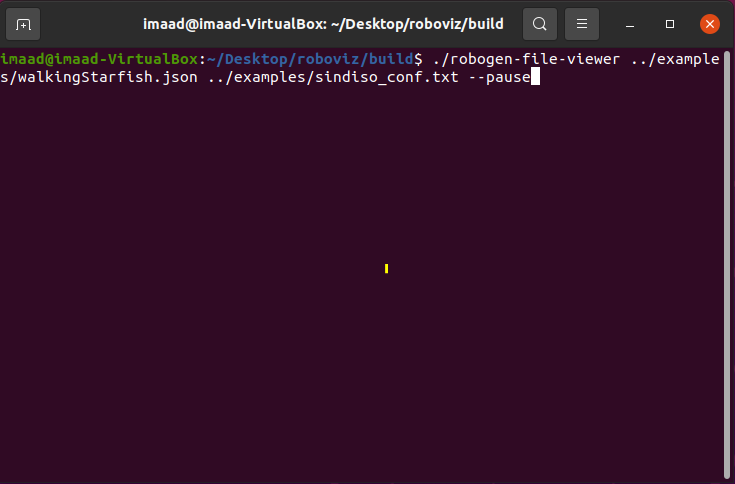
\includegraphics[width=0.8\textwidth]{run}
    \caption{commands in terminal }
    \label{fig:commands-in-terminal}
\end{figure}

Once entered, the follwing screen should be displayed.
\begin{figure}[htpb]
    \centering
    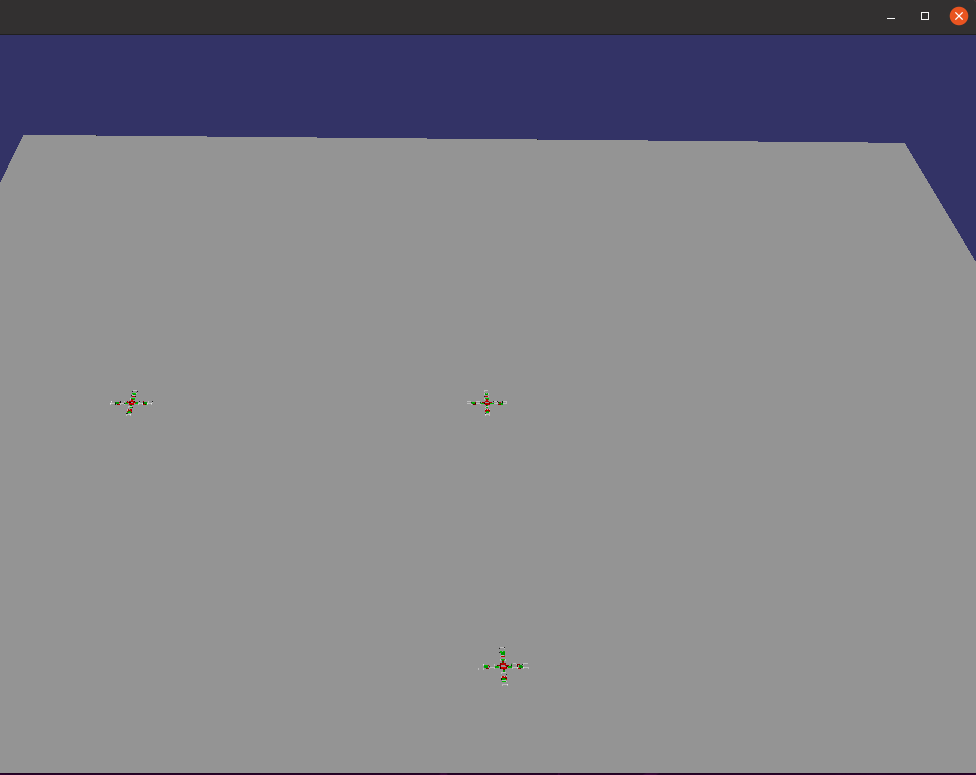
\includegraphics[width=0.8\textwidth]{visual1}
    \caption{Robots in Visualiser}
    \label{fig:robots-in-visualiser}
\end{figure}

